\documentclass[12pt]{article}
\usepackage[utf8]{inputenc}
\usepackage{lmodern}
\usepackage[T1]{fontenc}
\usepackage{booktabs}
\usepackage{amsmath}
\usepackage{enumitem}
\usepackage{graphicx}
\usepackage{fullpage}
\usepackage{siunitx}
\usepackage{fancyhdr}
\PassOptionsToPackage{hyphens}{url}
\usepackage[hyphens]{url}
\usepackage{color}
\usepackage{enumitem}
\usepackage{textcomp}
\usepackage[table,xcdraw]{xcolor}
\usepackage{geometry}
\usepackage{courier}
\usepackage{listings}
\usepackage{array}
\usepackage{amsthm}
\usepackage{mathdots}
\usepackage{amssymb}
\usepackage{minted}
\usepackage{wrapfig}
\usepackage{titlesec}
\usepackage{parskip}
\usepackage{accents}
\usepackage{gensymb}
\usepackage{indentfirst}
\usepackage{courier}
\usepackage{framed}
\usepackage{etoolbox}
\usepackage{titlesec}
\usepackage{appendix}
\usepackage{mdframed}
\usepackage{verbatim}
\usepackage{xspace}
\usepackage{hyperref}

\AtBeginEnvironment{subappendices}{%
	\section*{Appendix}
	\addcontentsline{toc}{section}{Appendices}
}
 %\lstset{language=C++,
%                basicstyle=\ttfamily,
%                keywordstyle=\color{blue}\ttfamily,
%                stringstyle=\color{red}\ttfamily,
%                commentstyle=\color{green}\ttfamily,
%                morecomment=[l][\color{magenta}]{\#}
%}
 \definecolor{keywordcolor}{rgb}{0,0,0.45}
\definecolor{stringcolor}{rgb}{0.45,0.45,0.45}
\definecolor{commentcolor}{rgb}{0,0.3,0}
 \lstset{
	language=C++,
	basicstyle=\footnotesize\ttfamily,
	numbers=left,
	%numberstyle=\tiny,
	frame=tb,
	columns=fullflexible,
	showstringspaces=false,
	breaklines=true,
	tabsize=4,
	keywordstyle=\color{keywordcolor}\footnotesize\bf\ttfamily,
	stringstyle=\color{stringcolor}\footnotesize\ttfamily,
	commentstyle=\color{commentcolor}\it\sffamily
}
% \lstset{basicstyle=\ttfamily,breaklines=true}
\lstloadlanguages{C++}
 %\renewcommand{\familydefault}{\sfdefault}
 \addtolength{\parskip}{\baselineskip}  
\newcommand{\urlwofont}[1]{\urlstyle{same}\url{#1}}
 \renewcommand{\arraystretch}{0.8}
\renewcommand{\headrulewidth}{0pt}
\renewcommand{\footrulewidth}{0pt}
 \newcommand{\imagewidth}{0.8\textwidth}
 \lhead{}
\chead{}
\rhead{}
\lfoot{}
\cfoot{\thepage}
\rfoot{}
 \geometry{
	top=0.9in,
	inner=0.7in,
	outer=0.7in,
	bottom=0.9in,
	headheight=2ex,
	headsep=1ex,
}
\pagestyle{fancy}
%\fancyhf{}
%\setlength{\headsep}{0.2in}
 \fancypagestyle{firststyle}
{
	\chead{}
	\setlength{\headsep}{0.0in}
}
\hypersetup{
	unicode=true,
	colorlinks=true,
	linkcolor=blue,
	citecolor=black,
	filecolor=black,
	urlcolor=blue
}
 \begingroup
\makeatletter
\@for\theoremstyle:=definition,remark,plain\do{%
	\expandafter\g@addto@macro\csname th@\theoremstyle\endcsname{%
		\addtolength\thm@preskip\parskip
	}%
}
\endgroup
 \newtheorem{thm}{Theorem}[section]
\newtheorem{lemma}{Lemma}[section]
\newtheorem{claim}{Claim}[section]
\newtheorem{proposition}{Proposition}[section]
%\theoremstyle{empty}
\newtheorem*{namedthm}{Theorem}
 % indention size
%\setlength{\parindent}{19pt}
\setlength{\parindent}{0pt}
 % paragraph spacing
\setlength{\parskip}{1em}
 % line spacing
\linespread{1}
 %\setcounter{tocdepth}{1}
 % Documenting starts here! Please do not change above! 
 \newcommand{\mytitle}
{
	\textbf {
		inzva Algorithm Programme 2018-2019\\ \ \\
		Bundle 6 \\ \ \\ 
		Veri Yap{\i}lar{\i}- 1 \\ \ \\
	}
}
 \title{\vspace{-2em}\mytitle\vspace{-0.3em}}
 \author{
	\textbf{Editor}\\
	Tahsin Enes Kuru  \\ \ \\ 
	\textbf{Reviewers} \\ 
	Baha Eren Yald{\i}z \\
    Burak Bu\u{g}rul
}
 \date{}
\begin{document}
	
	\begin{figure}
		\centering
		
\includegraphics[width=\linewidth/4]{inzva-logo.png}
		\label{fig:inzva}
	\end{figure}
	\maketitle
	
	\cleardoublepage
	\tableofcontents
	\markboth{Table of Contents}{}
	\cleardoublepage
	
	\section{Giri\c{s}}

    Bilgisayar biliminde veri yap{\i}lar{\i}, belirli bir eleman k\"{u}mesi \"{u}zerinde verimli bir \c{s}eklide bilgi edinmemize ayn{\i} zamanda bu elemanlar \"{u}zerinde de\u{g}i\c{s}iklikler yapabilmemize olanak sa\u{g}layan yap{\i}lard{\i}r. \c{C}al{\i}\c{s}ma prensipleri genellikle elemanlar{\i}n de\u{g}erlerini belirli bir kurala g\"{o}re saklamak daha sonra bu yap{\i}lar{\i} kullanarak elemanlar hakk{\i}nda sorulara (Bir dizinin belirli bir aral{\i}\u{g}{\i}ndaki en k\"{u}\c{c}\"{u}k say{\i} gibi) cevap aramakt{\i}r.
	\section{Dinamik Veri Yap{\i}lar{\i}}
	
	\subsection{Linked List}
	
	Linked List veri yap{\i}s{\i}nda elemanlar, her eleman kendi de\u{g}erini ve bir sonraki eleman{\i}n adresini tutacak \c{s}ekilde saklan{\i}r. Yap{\i}daki elemanlar ba\c{s} elemandan(head) ba\c{s}lanarak son elemana(tail) gidecek \c{s}ekilde gezilebilir. Diziye kar\c{s}{\i}n avantaj{\i} haf{\i}zan{\i}n dinamik bir \c{s}ekilde kullan{\i}lmas{\i}d{\i}r. Bu veri yap{\i}s{\i}nda uygulanabilecek i\c{s}lemler:
	
	\begin{itemize}
        \item Veri yap{\i}s{\i}n{\i}n sonuna eleman ekleme.
        \item Anl{\i}k veri yap{\i}s{\i}n{\i} ba\c{s}tan(head) sona(tail) gezme.
    \end{itemize}

	\begin{figure}[h]
		\centering
		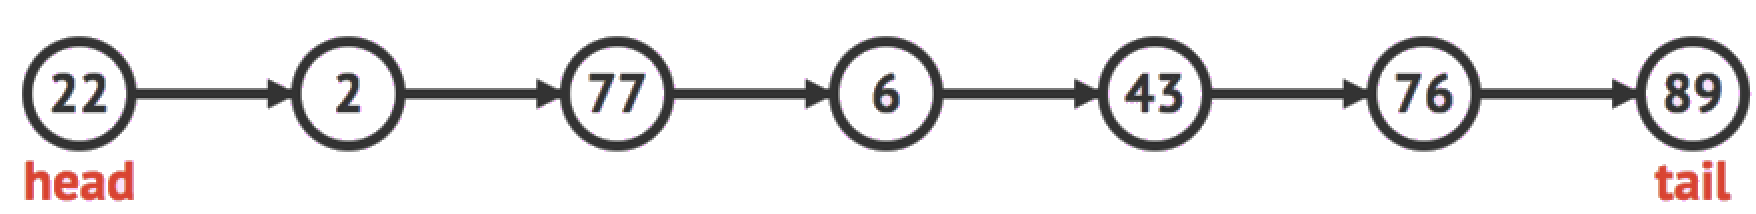
\includegraphics[width=\linewidth/1]{linkedlist.png}
		\label{fig:linkedlist}
        \caption{\"{O}rnek bir Linked List yap{\i}s{\i}}
	\end{figure}        
    
    \clearpage

    \begin{minted}[frame=lines,linenos,fontsize=\footnotesize]{c++}
// Her bir elemani tutacak struct olusturuyoruz.
struct node
{
  int data;
  node *next;
};
node *head, *tail;

void push_back(int x) {
  // Yeni elemanimizi hafizada olusturuyoruz.
  node *t = (node*)malloc(sizeof(node)); 
  t -> data = x; // Elemanin verisini atiyoruz.
  t -> next = NULL; // Sona ekledigimizden sonraki elemanina NULL atiyoruz.

  // Eger veri yapimiza hic eleman eklenmediyse head 
  // ve tail elemanlarini olusturuyoruz.
  if(head == NULL && tail == NULL) {
    head = t;
    tail = t;
  }
  // Eklenmisse yeni tail elemanimizi guncelliyoruz.
  else {
    tail -> next = t; 
    tail = t;
  }
}

void print() {
  // Dizideki tum elemanlari geziyoruz.
  node *t = head;
  while(t != NULL) {
    printf("%d ", t -> data);
    t = t -> next;
  }
}
    \end{minted}

	\subsection{Stack}
    
    Stack veri yap{\i}s{\i}nda elemanlar yap{\i}ya son giren ilk \c{c}{\i}kar (LIFO) kural{\i}na uygun olacak \c{s}ekilde saklan{\i}r. Bu veri yap{\i}s{\i}nda uygulayabildi\u{g}imiz i\c{s}lemler:
    
    \begin{itemize}
        \item Veri yap{\i}s{\i}n{\i}n en \"{u}st\"{u}ne eleman ekleme.
        \item Veri yap{\i}s{\i}n{\i}n en \"{u}st\"{u}ndeki elemana eri\c{s}im.
        \item Veri yap{\i}s{\i}n{\i}n en \"{u}st\"{u}ndeki eleman{\i} silme.
    \end{itemize}
    
    c++ dilindeki stl k\"{u}t\"{u}phanesinde bulunan haz{\i}r stack yap{\i}s{\i}n{\i}n kullan{\i}m{\i} a\c{s}a\u{g}{\i}daki gibidir.
    
    \begin{minted}[frame=lines,linenos,fontsize=\footnotesize]{c++}
int main() {
  stack < int > st;
  st.push(5); // Stack'in en ustune 5'i ekler. Stack'in yeni hali: {5}
  st.push(7); // Stack'in en ustune 7'yi ekler. Stack'in yeni hali: {7,5}
  st.push(6); // Stack'in en ustune 6'yiekler. Stack'in yeni hali : {6, 7, 5}
  st.pop(); //Stack'in en ustundeki elemani siler. Stack'in yeni hali : {7, 5}
  st.push(1); // Stack'in en ustune 1'i ekler. Stack'in yeni hali : {1 7, 5}
  cout << st.top() << endl; // Stack'in en ustundeki elemana erisir. Ekrana 1 yazirir.  
}
    \end{minted}
	
	\subsection{Queue}

    Queue veri yap{\i}s{\i}nda elemanlar yap{\i}ya ilk giren ilk \c{c}{\i}kar (FIFO) kural{\i}na uygun olacak \c{s}ekilde saklan{\i}r. Bu veri yap{\i}s{\i}nda uygulayabildigimiz i\c{s}lemler:
    
    \begin{itemize}
        \item Veri yap{\i}s{\i}n{\i}n en \"{u}st\"{u}ne eleman ekleme.
        \item Veri yap{\i}s{\i}n{\i}n en alt{\i}ndaki eleman{\i}na eri\c{s}im.
        \item Veri yap{\i}s{\i}n{\i}n en alt{\i}ndaki eleman{\i} silme.
    \end{itemize}
    
    c++ dilindeki stl k\"{u}t\"{u}phanesinde bulunan haz{\i}r queue yap{\i}s{\i}n{\i}n kullan{\i}m{\i} a\c{s}a\u{g}{\i}daki gibidir.
    
    \begin{minted}[frame=lines,linenos,fontsize=\footnotesize]{c++}
int main() {
  queue < int > q;
  q.push(5); // queue'in en ustune 5'i ekler. queue'in yeni hali: {5}
  q.push(7); // queue'in en ustune 7'yi ekler. queue'in yeni hali: {7,5}
  q.push(6); // queue'in en ustune 6'yi ekler. queue'in yeni hali : {6, 7, 5}
  q.pop(); //queue'in en altindaki elemani siler. queue'in yeni hali : {6,7}
  q.push(1); // queue'in en ustune 1'i ekler. queue'in yeni hali : {1,6,7}
  cout << q.front() << endl; // queue'in en ustundeki elemana erisir. Ekrana 7 yazirir.   
}
    \end{minted}
	
	\subsection{Deque}
	
	Deque veri yap{\i}s{\i} stack ve queue veri yap{\i}lar{\i}na g\"{o}re daha kapsaml{\i}d{\i}r.
    Bu veri yap{\i}s{\i}nda yap{\i}n{\i}n en \"{u}st\"{u}ne eleman eklenebilirken ayn{\i} zamanda en alt{\i}na da eklenebilir. Ayn{\i} \c{s}ekilde yap{\i}n{\i}n hem en \"{u}st\"{u}ndeki eleman{\i}na hem de en alttaki eleman{\i}na eri\c{s}im ve silme i\c{s}lemleri uygulanabilir. Bu veri yap{\i}s{\i}nda uyguluyabildi\u{g}imiz i\c{s}lemler:

    \begin{itemize}
        \item Veri yap{\i}s{\i}n{\i}n en \"{u}st\"{u}ne eleman ekleme.
        \item Veri yap{\i}s{\i}n{\i}n en alt{\i}na eleman ekleme.
        \item Veri yap{\i}s{\i}n{\i}n en \"{u}st\"{u}ndeki eleman{\i}na eri\c{s}im.
        \item Veri yap{\i}s{\i}n{\i}n en alt{\i}ndaki eleman{\i}na eri\c{s}im.
        \item Veri yap{\i}s{\i}n{\i}n en \"{u}st\"{u}ndeki eleman{\i} silme.
        \item Veri yap{\i}s{\i}n{\i}n en alt{\i}ndaki eleman{\i} silme.
    \end{itemize}
    
    c++ dilindeki stl k\"{u}t\"{u}phanesinde bulunan haz{\i}r dequeu yap{\i}s{\i}n{\i}n kullan{\i}m{\i} a\c{s}a\u{g}{\i}daki gibidir.    
    
    \begin{minted}[frame=lines,linenos,fontsize=\footnotesize]{c++}
int main() {
  deque < int > q;
  q.push_front(5); // deque'nin en altina 5'i ekler.
  q.push_back(6); // deque'nin en ustune 6'yi ekler.
  int x = q.front(); // deque'nin en altindaki elemanina erisim.
  int y = q.back(); // deque'nin en ustundeki elemanina erisim.
  q.pop_front(); // deque'nin en altindaki elemanini silme.
  q.pop_back(); // deque'nin en ustundeki elemanini silme.
}
    \end{minted}
    \cleardoublepage

	\section{Prefix Sum}
	
	Prefix Sum dizisi bir dizinin prefixlerinin toplamlar{\i}yla olu\c{s}turulan bir veri yap{\i}s{\i}d{\i}r. Prefix sum dizisinin i indeksli eleman{\i} girdi dizisindeki 1 indeksli elemandan i indeksli elemana kadar olan elemanlar{\i}n toplam{\i}na e\c{s}it olacak \c{s}ekilde kurulur. Ba\c{s}ka bir de\u{g}i\c{s}le: $$sum_i = \sum_{j=1}^{i} {a_j} $$ \"{O}rnek bir $A$ dizisi i\c{c}in prefix sum dizisi \c{s}u \c{s}ekilde kurulmal{\i}d{\i}r:

    \begin{table}[h]
    \centering
    \begin{tabular}{|c|c|c|c|c|c|}
    \hline
    \textbf{A Dizisi} & 4 & 6 & 3 & 12 & 1 \\ \hline
    \textbf{Prefix Sum Dizisi} & 4 & 10 & 13 & 25 & 26 \\ \hline
     & \cellcolor[HTML]{F8FF00}4 & \cellcolor[HTML]{F8FF00}4 + 6 & \cellcolor[HTML]{F8FF00}4 + 6 + 3 & \cellcolor[HTML]{F8FF00}4 + 6 + 3 + 12 & \cellcolor[HTML]{F8FF00}4 + 6 + 3 + 12 + 1 \\ \hline
    \end{tabular}
    \end{table}

	Prefix sum dizisini kullanarak herhangi bir $[l,r]$ aral{\i}\u{g}{\i}ndaki elemanlar{\i}n toplam{\i}n{\i} \c{s}u \c{s}ekilde kolayl{\i}kla elde edebiliriz:
	
    $$sum_r = \sum_{j=1}^{r} {a_j} $$ 
    $$sum_{l - 1} = \sum_{j=1}^{l - 1} {a_j} $$ 
	$$sum_r - sum_{l-1} = \sum_{j=l}^{r} {a_j}$$
	
	\subsection{\"{O}rnek Kod Par\c{c}alar{\i}}
	
    $sum_i = sum_{i -1} + a_i$ e\c{s}itli\u{g}i kolayca g\"{o}r\"{u}l\"{u}r. Ve bu e\c{s}itli\u{g}i kullanarak Prefix Sum dizisini girdi dizisindeki elemanlar{\i} s{\i}rayla gezerek kurabiliriz.
	
    \begin{minted}[frame=lines,linenos,fontsize=\footnotesize]{c++}
int n,sum[N],a[N];
// a dizisi girdi dizimiz, sum dizisi de prefix sum dizimiz olsun.

void build() {
  for (int i = 1 ; i <= n ; i++)
    sum[i] = sum[i - 1] + a[i];
  return;
}

int query(int l,int r) {
  return sum[r] - sum[l - 1];
}
    \end{minted}

	\subsection{Zaman Karma\c{s}{\i}kl{\i}\u{g}{\i}}
	
    Prefix sum dizisini kurma i\c{s}lemimizin zaman ve haf{\i}za karma\c{s}{\i}kl{\i}\u{g}{\i} $O(N)$. Her sorguya da $O(1)$ karma\c{s}{\i}kl{\i}kta cevap verebiliyoruz. 

    Prefix sum veri yap{\i}s{\i} ile ilgili problem: \href{https://uva.onlinejudge.org/index.php?option=com_onlinejudge&Itemid=8&category=24&page=show_problem&problem=1474}{Link}.
    \cleardoublepage

	\section{Sparse Table}

    Sparse Table aral{\i}klardaki elemanlar{\i}n toplam{\i}, minimumu, maksimumu ve eboblar{\i} gibi sorgulara $O(logN)$ zaman karma\c{s}{\i}kl{\i}\u{g}{\i}nda cevap alabilmemizi sa\u{g}layan bir veri yap{\i}s{\i}d{\i}r. Baz{\i} tip sorgular (aral{\i}ktaki minimum, maksimum say{\i}y{\i} bulma gibi) ise $O(1)$ zaman karma\c{s}{\i}kl{\i}\u{g}{\i}nda yapmaya uygundur.
    
    Bu veri yap{\i}s{\i} durumu de\u{g}i\c{s}meyen, sabit bir veri \"{u}zerinde \"{o}n i\c{s}lemler yaparak kurulur. Dinamik veriler i\c{c}in kullan{\i}\c{s}l{\i} de\u{g}ildir. Veri \"{u}zerinde herhangi bir de\u{g}i\c{s}iklik durumda Sparse Table tekrardan kurulmal{\i}d{\i}r. Bu da maliyetli bir durumdur.
    
    \subsection{Yap{\i}s{\i} ve Kurulu\c{s}u}
    
    Sparse table iki bouyutlu bir dizi \c{s}eklinde, $O(NlogN)$ haf{\i}za karma\c{s}{\i}kl{\i}\u{g}{\i}na sahip bir veri yap{\i}s{\i}d{\i}r. Dizinin her eleman{\i}ndan 2'nin kuvvetleri uzakl{\i}ktaki elemanlara kadar olan cevaplar Sparse tableda saklan{\i}r. $ST_{x,i}$, $x$ indeksli elemandan $x + 2^i$ indeksli elemana kadar olan aral{\i}\u{g}{\i}n cevab{\i}n{\i} saklayacak \c{s}ekilde sparse table kurulur.
    
    \begin{minted}[frame=lines,linenos,fontsize=\footnotesize]{c++}
//Toplam sorgusu icin kurulmus Sparse Table Yapisi
void build() {

  for (int i = 1 ; i <= n ; i++) {
    // [i,i] araliginin cevabi dizinin i indeksli elemanina esittir.
    ST[i][0] = a[i];
  }

  for (int i = 1 ; i <= LOG ; i++)
    for (int j = 1 ; j <= n ; j++) {
      // [i,i+2^(j)] araliginin cevabi
      // [i,i+2^(j - 1) - 1] araligi ile [i+2^(j - 1),i+2^j] araliginin
      // cevaplarinin birlesmesiyle elde edilir
      ST[i][j] = ST[i][j - 1] + ST[i + (1 << (j - 1))][j - 1];
    }

  return;
}
    \end{minted}
    \cleardoublepage
    
    \subsection{Sorgu Algoritmas{\i}}
    
    Herhangi bir $[l,r]$ aral{\i}\u{g}{\i} i\c{c}in sorgu algoritmas{\i} s{\i}ras{\i}yla \c{s}u \c{s}ekilde \c{c}al{\i}\c{s}{\i}r:
    
    \begin{itemize}
        \item $[l,r]$ aral{\i}\u{g}{\i}n{\i} cevaplar{\i}n{\i} \"{o}nceden hesaplad{\i}\u{g}{\i}m{\i}z aral{\i}klara par\c{c}ala. (Sadece $2$'nin kuvveti uzunlu\u{g}unda par\c{c}alar{\i}n cevaplar{\i}n{\i} saklad{\i}\u{g}{\i}m{\i}z i\c{c}in aral{\i}\u{g}{\i}m{\i}z{\i} $2$'nin kuvveti uzunlu\u{g}unda aral{\i}klara ay{\i}rmal{\i}y{\i}z. $[l,r]$ aral{\i}\u{g}{\i}n{\i}n uzunlu\u{g}unun iklik tabanda yazd{\i}\u{g}{\i}m{\i}zda hangi aral{\i}klara par\c{c}alamam{\i}z gerekti\u{g}ini bulmu\c{s} oluruz.) 
        
        \item Bu aral{\i}klardan gelen cevaplar{\i} birle\c{s}tirerek $[l,r]$ aral{\i}\u{g}{\i}n{\i}n cevab{\i}n{\i} hesapla.
        
    \end{itemize}
    
    Herhangi bir aral{\i}\u{g}{\i}n uzunlu\u{g}unun ikilik tabandaki yaz{\i}l{\i}\c{s}{\i}ndaki $1$ rakamlar{\i}n{\i}n say{\i}s{\i} en fazla $logN$ olabilece\u{g}inden par\c{c}alayaca\u{g}{\i}m{\i}z aral{\i}k say{\i}s{\i} da en fazla $logN$ olur. Dolay{\i}s{\i}yla sorgu i\c{s}lemimiz $O(logN)$ zaman karma\c{s}{\i}kl{\i}\u{g}{\i}nda \c{c}al{\i}\c{s}{\i}r. 
    
    \"{O}rne\u{g}in: $[4,17]$ aral{\i}\u{g}{\i}n{\i}n cevab{\i}n{\i} hesaplamak i\c{c}in algoritmam{\i}z $[4,17]$ aral{\i}\u{g}{\i}n{\i} $[4,11]$,$[12,15]$ ve $[16,17]$ aral{\i}klar{\i}na ay{\i}r{\i}r ve bu $3$ aral{\i}ktan gelen cevaplar{\i} birle\c{s}tirerek istenilen cevab{\i} hesaplar.
    
    \begin{minted}[frame=lines,linenos,fontsize=\footnotesize]{c++}
//toplam sorgusu

int query(int l,int r) {

  int res = 0;

  for (int i = LOG ; i >= 0 ; i--) {
    // her seferinde uzunlugu r - l + 1 gecmeyecek
    // en buyuk araligin cevabi ekleyip l'i o araligin sonuna cekiyoruz.
    if (l + (1 << i) <= r) {
      res += ST[l][i];
      l += (1 << i);
    }
  }

  return res;

}
    \end{minted}    

    \subsection{Minimum ve Maksimum Sorgu}
    
    Sparse Table veri yap{\i}s{\i}n{\i}n di\u{g}er veri yap{\i}lar{\i}ndan farkl{\i} olarak $O(1)$ zaman karma\c{s}{\i}kl{\i}\u{g}{\i}nda aral{\i}klarda  minimum veya maksimum sorgusu yapabilmesi en avantajl{\i} \"{o}zelli\u{g}idir.

    Herhangi bir aral{\i}\u{g}{\i}n cevab{\i}n{\i} hesaplarken bu aral{\i}ktaki herhangi bir eleman{\i} birden fazla kez de\u{g}erlendirmemiz cevab{\i} etkilemez. Bu durum aral{\i}\u{g}{\i}m{\i}z{\i} 2'nin kuvveti uzunlu\u{g}unda maksimum 2 adet aral{\i}\u{g}a b\"{o}lebilmemize ve bu aral{\i}klar{\i}n cevaplar{\i}n{\i} $O(1)$ zaman karma\c{s}{\i}kl{\i}\u{g}{\i}nda birle\c{s}tirebilmemize olanak sa\u{g}lar.
    
    \begin{minted}[frame=lines,linenos,fontsize=\footnotesize]{c++}
int RMQ(int l,int r) {
  // log dizisinde her sayinin log2 degerleri sakldir.
  int j = log[r - l + 1];
  return min(ST[l][j], ST[r - (1 << j) + 1][j]);  
}
    \end{minted}
    
    Sparse Table veri yap{\i}s{\i} ile ilgili problem: \href{https://www.spoj.com/problems/RMQSQ/}{Link}.

    \cleardoublepage
	
	\section{Binary Indexed Tree}
	
	Fenwick tree olarak da bilinen Binary Indexed Tree, Prefix sum ve Sparse Table yap{\i}lar{\i}na benzer bir yap{\i}da olup dizi \"{u}zerinde de\u{g}i\c{s}iklik yapabilmemize olanak sa\u{g}layan bir veri yap{\i}s{\i}d{\i}r. Fenwick Tree'nin di\u{g}er veri yap{\i}lar{\i}na g\"{o}re en b\"{u}y\"{u}k avantaj{\i} pratikte daha h{\i}zl{\i} olmas{\i} ve haf{\i}za karma\c{s}{\i}kl{\i}\u{g}{\i}n{\i}n $O(N)$ olmas{\i}d{\i}r. Ancak Fenwick Tree'de sadece prefix cevaplar{\i} saklayabildi\u{g}imizden aral{\i}klarda minimum, maksimum ve en b\"{u}y\"{u}k ortak b\"{o}len gibi baz{\i} sorgular{\i}n cevaplar{\i}n{\i} elde edemeyiz.
	
	\subsection{Yap{\i}s{\i} ve Kurulu\c{s}u}
	
	$g(x)$, $x$ say{\i}s{\i}n{\i}n bit g\"{o}steriminde yaln{\i}zca en sa\u{g}daki bitin 1 oldu\u{g}u tamsay{\i} olsun. \"{O}rne\u{g}in $20$'nin bit g\"{o}sterimi $(10100)_2$ oldu\u{g}undan $g(20)=4$'t\"{u}r. \c{C}\"{u}nk\"{u} ilk kez sa\u{g}dan $3.$ bit $1$'dir ve $(00100)_2=4$'t\"{u}r.  Fenwick Tree'nin x indeksli d\"{u}\u{g}\"{u}m\"{u}nde, $x -g(x)+1$ indeksli elemandan $x$ indeksli elemana kadar olan aral{\i}\u{g}{\i}n cevab{\i}n{\i} saklayacak \c{s}eklide kurulur.
	
	\begin{figure}[h]
		\centering
		\includegraphics[width=\linewidth/1]{fenwick.png}
		\label{fig:fenwick}
        \caption{$a = [62,6,85,60,39,47,60,16,17]$ dizisinde toplam sorgusu i\c{c}in kurulmu\c{s} Fenwick Tree yap{\i}s{\i}}
	\end{figure}
	
	\clearpage

    \subsection{Sorgu Algoritmas{\i}}
    
    Herhangi bir $[1,x]$ aral{\i}\u{g}{\i} i\c{c}in sorgu algoritmas{\i} s{\i}ras{\i} ile \c{s}u \c{s}eklide \c{c}al{\i}\c{s}{\i}r.
    
    \begin{enumerate}
        \item Arad{\i}\u{g}{\i}m{\i}z cevaba $[x - g(x) + 1,x]$ aral{\i}\u{g}{\i}n{\i}n cevab{\i}n{\i} ekle.
        \item x'in de\u{g}erini $x - g(x)$ yap. E\u{g}er x'in yeni de\u{g}eri $0$'dan b\"{u}y\"{u}k ise 1.i\c{s}lemden hesaplamaya devam et.  
    \end{enumerate}
    
    $[1,x]$ aral{\i}\u{g}{\i}n{\i}n cevab{\i}n{\i} hesaplamak i\c{c}in yap{\i}lan i\c{s}lem say{\i}s{\i} $x$ say{\i}s{\i}n{\i}n $2$'lik tabandaki yaz{\i}l{\i}\c{s}{\i}ndaki $1$ say{\i}s{\i}na e\c{s}ittir. \c{C}\"{u}nk\"{u} her d\"{o}ng\"{u}de x'den $2$'lik tabandaki yaz{\i}l{\i}\c{s}{\i}ndaki en sa\u{g}daki $1$ bitini \c{c}{\i}kart{\i}yoruz. Dolay{\i}s{\i}yla sorgu i\c{s}lemimiz $O(logN)$ zaman karma\c{s}{\i}kl{\i}\u{g}{\i}nda \c{c}al{\i}\c{s}{\i}r. $[l,r]$ aral{\i}\u{g}{\i}n{\i}n cevab{\i}n{\i} da $[1,r]$ aral{\i}\u{g}{\i}n{\i}n cevab{\i}ndan $[1,l - 1]$ aral{\i}\u{g}{\i}n{\i}n cevab{\i}n{\i} \c{c}{\i}kararak kolay bir \c{s}ekilde elde edebiliriz.
    
    \fbox{
        \parbox{\textwidth}
        {
        NOT: $g(x)$ de\u{g}erini bitwise operat\"{o}rlerini kullanarak a\c{s}a\u{g}{\i}daki  e\c{s}itlikle kolay bir \c{s}ekilde hesaplayabiliriz: $$g(x) = x \& (-x)$$
        }
    }
    
    \subsection{Eleman G\"{u}ncelleme Algoritmas{\i}}
    
    Dizideki $x$ indeksli eleman{\i}n{\i}n de\u{g}erini g\"{u}ncellemek  i\c{c}in kullan{\i}lan algoritma \c{s}u \c{s}eklide \c{c}al{\i}\c{s}{\i}r.
    
    \begin{itemize}
        \item A\u{g}a\c{c}ta $x$ indeksli eleman{\i} i\c{c}eren t\"{u}m d\"{u}\u{g}\"{u}mlerin de\u{g}erlerini g\"{u}ncelle.
    \end{itemize}
    
    Fenwick Tree'de x indeksli eleman{\i} i\c{c}eren maksimum $logN$ tane aral{\i}k oldu\u{g}undan g\"{u}ncelleme algoritmas{\i} $O(logN)$ zaman karma\c{s}{\i}kl{\i}\u{g}{\i}nda \c{c}al{\i}\c{s}{\i}r.
    
    \clearpage
    
    \subsection{\"{O}rnek Kod Par\c{c}alar{\i}}
    
    \begin{minted}[frame=lines,linenos,fontsize=\footnotesize]{c++}
    
int n,tree[N],a[N];

void add(int val,int x) { // x indeksli elemanin degerini val degeri kadar artirir.
  while(x <= n) {
    tree[x] += val;
    x += x & (-x);
  }
  return;
}

int sum(int x) { // 1 indeksli elemandan x indeksli elemana
  int res = 0; // kadar olan sayilarin toplamini verir.
  while(x >= 1) {
    res += tree[x];
    x -= x & (-x);
  }
  return res;
}

int query(int l,int r) { // [l,r] araligindaki elemanlarin toplamini verir.
  return sum(r) - sum(l - 1);
}

void build() { // a dizisi uzerine fenwick tree yapisini kuruyoruz.
  for (int i = 1 ; i <= n ; i++)
    add(a[i],i);
  return;
}

    \end{minted}
    
    \subsection{Aral{\i}k G\"{u}ncelleme ve Eleman Sorgu}

    Bir $a$ dizisi \"{u}zerinde i\c{s}lemler yapaca\u{g}{\i}m{\i}z{\i} varsayal{\i}m daha sonra $a$ dizisi $b$ dizisinin prefix sum dizisi olacak \c{s}ekilde bir $b$ dizisi tan{\i}mlayal{\i}m. Ba\c{s}ka bir de\u{g}i\c{s}le $a_i = \sum_{j=1}^{i} {b_j} $ olmal{\i}d{\i}r. Sonradan olu\c{s}turdu\u{g}umuz $b$ dizisi \"{u}zerine fenwick tree yap{\i}s{\i}n{\i} kural{\i}m. $[l,r]$ aral{\i}\u{g}{\i}ndaki her elemana
    $x$ de\u{g}erini eklememiz i\c{c}in uygulamam{\i}z gereken i\c{s}lemler:
    
    \begin{itemize}
        \item $b_l$ de\u{g}erini $x$ kadar art{\i}r. B\"{o}ylelikle $l$ indeksli elemandan dizinin sonuna kadar t\"{u}m elemanlar{\i}n de\u{g}eri $x$ kadar artm{\i}\c{s} olur.
        \item $b_{r + 1}$ de\u{g}erini $x$ kadar azalt. B\"{o}ylelikle $r + 1$ indeksli elemandan dizinin sonuna kadar t\"{u}m elemanlar{\i}n de\u{g}eri $x$ kadar azalm{\i}\c{s} olur. Bu i\c{s}lemelerin sonucunda sadece $[l,r]$ aral{\i}\u{g}{\i}ndaki elemanlar{\i}n de\u{g}eri $x$ kadar artm{\i}\c{s} olur.
    \end{itemize}
    
    \subsubsection{\"{O}rnek Kod Par\c{c}alar{\i}}
    
    \begin{minted}[frame=lines,linenos,fontsize=\footnotesize]{c++}
int n,a[N],b[N];

void add(int val,int x) { // x indeksli elemanin degerini val degeri kadar artirir.
  while(x <= n) {
    tree[x] += val;
    x += x & (-x);
  }
  return;
}

int sum(int x) { // 1 indeksli elemandan x indeksli elemana
  int res = 0; // kadar olan sayilarin toplamini verir.
  while(x >= 1) {
    res += tree[x];
    x -= x & (-x);
  }
  return res;
}
void build() {
  for (int i = 1 ; i <= n ; i++)
    b[i] = a[i] - a[i - 1]; // b dizisini olusturuyoruz.

  for (int i = 1 ; i <= n ; i++)
    add(b[i],i); // b dizisi uzerine fenwick tree kuruyoruz.
}

void update(int l,int r,int x) {
  add(x,l);
  add(-x,r + 1);
}

void query(int x) {
  return sum(x);
}

    \end{minted}
    
    Fenwick Tree veri yap{\i}s{\i} ile ilgili problem: \href{https://www.spoj.com/problems/CSUMQ/}{Link}.
    \cleardoublepage

	\section{SQRT Decomposition}
	
	Square Root Decomposition algoritmas{\i} dizi \"{u}zerinde $O(\sqrt{N})$ zaman karma\c{s}{\i}kl{\i}\u{g}{\i}nda sorgu yapabilmemize ve $O(1)$ zaman karma\c{s}{\i}kl{\i}\u{g}{\i}nda ise de\u{g}i\c{s}iklik yapabilmemize olanak sa\u{g}layan bir veri yaps{\i}d{\i}r.
	
	\subsection{Yap{\i}s{\i} ve Kurulu\c{s}u}
	
	Dizinin elemanlar{\i} her biri yakla\c{s}{\i}k $O(\sqrt{N})$ uzunlu\u{g}unda bloklar halinde par\c{c}alan{\i}r. Her bir blo\u{g}un cevab{\i} ayr{\i} ayr{\i} hesaplan{\i}r ve bir dizide saklan{\i}r.
	
    \begin{table}[h]
    \centering
    \begin{tabular}{|c|c|c|c|c|c|c|c|c|c|c|c|c|c|c|c|c|}
    \hline
    Bloklar{\i}n Cevaplar{\i}   & \multicolumn{4}{c|}{21} & \multicolumn{4}{c|}{13} & \multicolumn{4}{c|}{50} & \multicolumn{4}{c|}{32} \\ \hline
    Dizideki Elemanlar     & 3    & 6   & 2   & 10   & 3    & 1    & 4   & 5   & 2   & 7    & 37   & 4   & 11   & 6    & 8   & 7   \\ \hline
    Elemanlar{\i}n \.{I}ndeksleri & 1    & 2   & 3   & 4    & 5    & 6    & 7   & 8   & 9   & 10   & 11   & 12  & 13   & 14   & 15  & 16  \\ \hline
    \end{tabular}
    \end{table}
    
	\"{O}rnek bir dizi \"{u}zerinde toplam sorgusu i\c{c}in kurulmu\c{s} SQRT Decompostion veri yap{\i}s{\i}.
	
    \begin{minted}[frame=lines,linenos,fontsize=\footnotesize]{c++}

void build() {
  for (int i = 1 ; i <= n ; i++) {
    if (i % sq == 1) { // sq = sqrt(n)
      t++; //yeni blok baslangici.
      st[t] = i; // t.blok i indisli elemanda baslar.
    }
    fn[t] = i; // t.blogun bitisini i indisli eleman olarak guncelliyoruz.
    wh[i] = t; // i indeksli eleman t.blogun icinde.
    sum[t] += a[i]; // t. blogun cevabina i indeksli elemani ekliyoruz.
  }
}

    \end{minted}
    
    \newpage

	\subsection{Sorgu Algoritmas{\i}}
	
	Herhangi bir $[l,r]$ aral{\i}\u{g}{\i} i\c{c}in sorgu algoritmas{\i} s{\i}ras{\i} ile \c{s}u \c{s}ekilde \c{c}al{\i}\c{s}{\i}r.
	
	\begin{enumerate}
	    \item Cevab{\i}n{\i} arad{\i}\u{g}{\i}m{\i}z aral{\i}\u{g}{\i}n tamamen kaplad{\i}\u{g}{\i} bloklar{\i}n cevab{\i}n{\i} cevab{\i}m{\i}za ekliyoruz.
	    
	    \item Tamamen kaplamad{\i}\u{g}{\i} bloklardaki aral{\i}\u{g}{\i}m{\i}z{\i}n i\c{c}inde olan elemanlar{\i} tek tek gezerek cevab{\i}m{\i}za ekliyoruz.
	    
	\end{enumerate}
	
     Cevab{\i}n{\i} arad{\i}\u{g}{\i}m{\i}z aral{\i}\u{g}{\i}n kapsad{\i}\u{g}{\i} blok say{\i}s{\i} en fazla $\sqrt{N}$ olabilece\u{g}inden $1.$ i\c{s}lem en fazla $\sqrt{N}$ kez \c{c}al{\i}\c{s}{\i}r. Tamamen kaplamad{\i}\u{g}{\i} ancak baz{\i} elemanlar{\i} i\c{c}eren en fazla $2$ adet blok olabilir. (Biri en solda di\u{g}eri en sa\u{g}da olacak \c{s}ekilde). Bu $2$ blok i\c{c}in de gezmemiz gereken eleman say{\i}s{\i} maksimum $2\sqrt{N}$ oldu\u{g}undan bir sorgu i\c{s}leminde en fazla $3\sqrt{N}$ i\c{s}lem yap{\i}l{\i}r dolay{\i}s{\i}yla sorgu i\c{s}lemimiz $O({\sqrt{N}})$ zaman karma\c{s}{\i}kl{\i}\u{g}{\i}nda cal{\i}\c{s}{\i}r.
    
    \begin{table}[h]
    \begin{tabular}{|c|c|c|c|c|c|c|c|c|c|c|c|c|c|c|c|c|}
    \hline
    Bloklar{\i}n Cevaplar{\i}    & \multicolumn{4}{c|}{21}                                        & \multicolumn{4}{c|}{\cellcolor[HTML]{FFFE65}13} & \multicolumn{4}{c|}{\cellcolor[HTML]{FFFE65}50} & \multicolumn{4}{c|}{32}                   \\ \hline
    Dizideki Elemanlar     & 3 & 6 & \cellcolor[HTML]{FFFE65}2 & \cellcolor[HTML]{FFFE65}10 & 3          & 1          & 4         & 5         & 2         & 7          & 37         & 4         & \cellcolor[HTML]{FFFE65}11 & 6  & 8  & 7  \\ \hline
    Elemanlar{\i}n \.{I}ndeksleri & 1 & 2 & 3                         & 4                          & 5          & 6          & 7         & 8         & 9         & 10         & 11         & 12        & 13                         & 14 & 15 & 16 \\ \hline
    \end{tabular}
    \end{table}
    
    \"{O}rnek dizideki $[3,13]$ aral{\i}\u{g}{\i}n{\i}n cevab{\i}n{\i} $2.$ ve $3.$ bloklar{\i}n cevaplar{\i} ile $3,4$ ve $11$ indeksli elemanlar{\i}n toplanmas{\i}yla elde edilir.
    
    \begin{minted}[frame=lines,linenos,fontsize=\footnotesize]{c++}
// [l,r] araligindaki elemanlarin toplamini hesaplayan fonksiyon.
int query(int l,int r) {

  int res = 0;

  if (wh[l] == wh[r]) { // l ve r ayni blogun icindeyse
    for (int i = l ; i <= r ; i++)
      res += a[i];
  }

  else {
    for (int i = wh[l] + 1 ; i <= wh[r] - 1 ; i++)
      res += sum[i]; // tamamen kapladigimiz bloklarin cevaplarini ekliyoruz.

    // tamamen kaplamadigimiz bloklardaki araligimiz icindeki
    // elemanlarin cevaplarini ekliyoruz.

    for (int i = st[wh[l]] ; i <= fn[wh[l]]; i++)
      if (i >= l && i <= r)
        res += a[i];

    for (int i = st[wh[r]] ; i <= fn[wh[r]] ; i++)
      if (i >= l && i <= r)
        res += a[i];
  }

  return res;
}
    \end{minted}    

    \subsection{Eleman G\"{u}ncelleme Algoritmas{\i}}
    
    Herhangi bir eleman{\i}n de\u{g}erini g\"{u}ncellerken o eleman{\i} i\c{c}eren blo\u{g}un de\u{g}erini g\"{u}ncellememiz yeterli olacakt{\i}r. Dolay{\i}s{\i}yla g\"{u}ncelleme i\c{s}lemimimiz $O(1)$ zaman karma\c{s}{\i}kl{\i}\u{g}{\i}nda \c{c}al{\i}\c{s}{\i}r. 
    
    \begin{minted}[frame=lines,linenos,fontsize=\footnotesize]{c++}
void update(int x,int val) {
  // x indeksli elemanin yeni degerini val degerine esitliyoruz.
  sum[wh[x]] -= a[x];
  a[x] = val;
  sum[wh[x]] += a[x];
}
    \end{minted} 
    
    SQRT Decomposition  veri yap{\i}s{\i} ile ilgili problem: \href{https://codeforces.com/contest/13/problem/E}{Link}.
    \cleardoublepage
    
	\section{Segment Tree}
	
    Segment Tree bir dizide $O(log N)$ zaman karma\c{s}{\i}kl{\i}\u{g}{\i}nda herhangi bir $[l,r]$ aral{\i}\u{g}{\i} icin minimum, maksimum, toplam gibi sorgulara cevap verebilmemize ve bu aral{\i}klar \"{u}zerinde g\"{u}ncelleme yapabilmemize olanak sa\u{g}layan bir veri yap{\i}s{\i}d{\i}r.
    
    Segment Tree'nin, Fenwick Tree ve Sparse Table yap{\i}lar{\i}ndan farkl{\i} olarak elemanlar \"{u}zerinde g\"{u}ncelleme yap{\i}labilmesi ve minimum, maksimum gibi sorgulara da olanak sa\u{g}lamas{\i} y\"{o}n\"{u}nden daha kullan{\i}\c{s}l{\i}d{\i}r. Ayr{\i}ca segment tree $O(N)$ haf{\i}za karma\c{s}{\i}kl{\i}\u{g}{\i}na sahipken Sparse Table yaps{\i}n{\i}nda 
    gereken haf{\i}za karma\c{s}{\i}kl{\i}\u{g}{\i} $O(NlogN)$'dir. 
    
    \subsection {Yap{\i}s{\i} ve Kurulu\c{s}u}
    
    Segment Tree, "Complete Binary Tree" yap{\i}s{\i}na sahiptir. Segment Tree'nin yaprak d\"{u}\u{g}\"{u}mlerinde dizinin elemanlar{\i} sakl{\i}d{\i}r ve bu d\"{u}\u{g}\"{u}mlerin atas{\i} olan her d\"{u}\u{g}\"{u}m kendi \c{c}ocu\u{g}u olan d\"{u}\u{g}\"{u}mlerinin cevaplar{\i}n{\i}n birle\c{s}mesiyle olu\c{s}ur. Bu sayede her d\"{u}\u{g}\"{u}mde belirli aral{\i}klar{\i}n cevaplar{\i} ve root d\"{u}\u{g}\"{u}m\"{u}nde t\"{u}m dizinin cevab{\i} saklan{\i}r. \"{O}rne\u{g}in toplam sorgusu i\c{c}in kurulmu\c{s} bir segment tree yap{\i}s{\i} i\c{c}in her d\"{u}\u{g}\"{u}m\"{u}n de\u{g}eri \c{c}ocuklar{\i}n{\i}n de\u{g}erleri toplam{\i}na e\c{s}ittir.

	\begin{figure}[h]
		\centering
		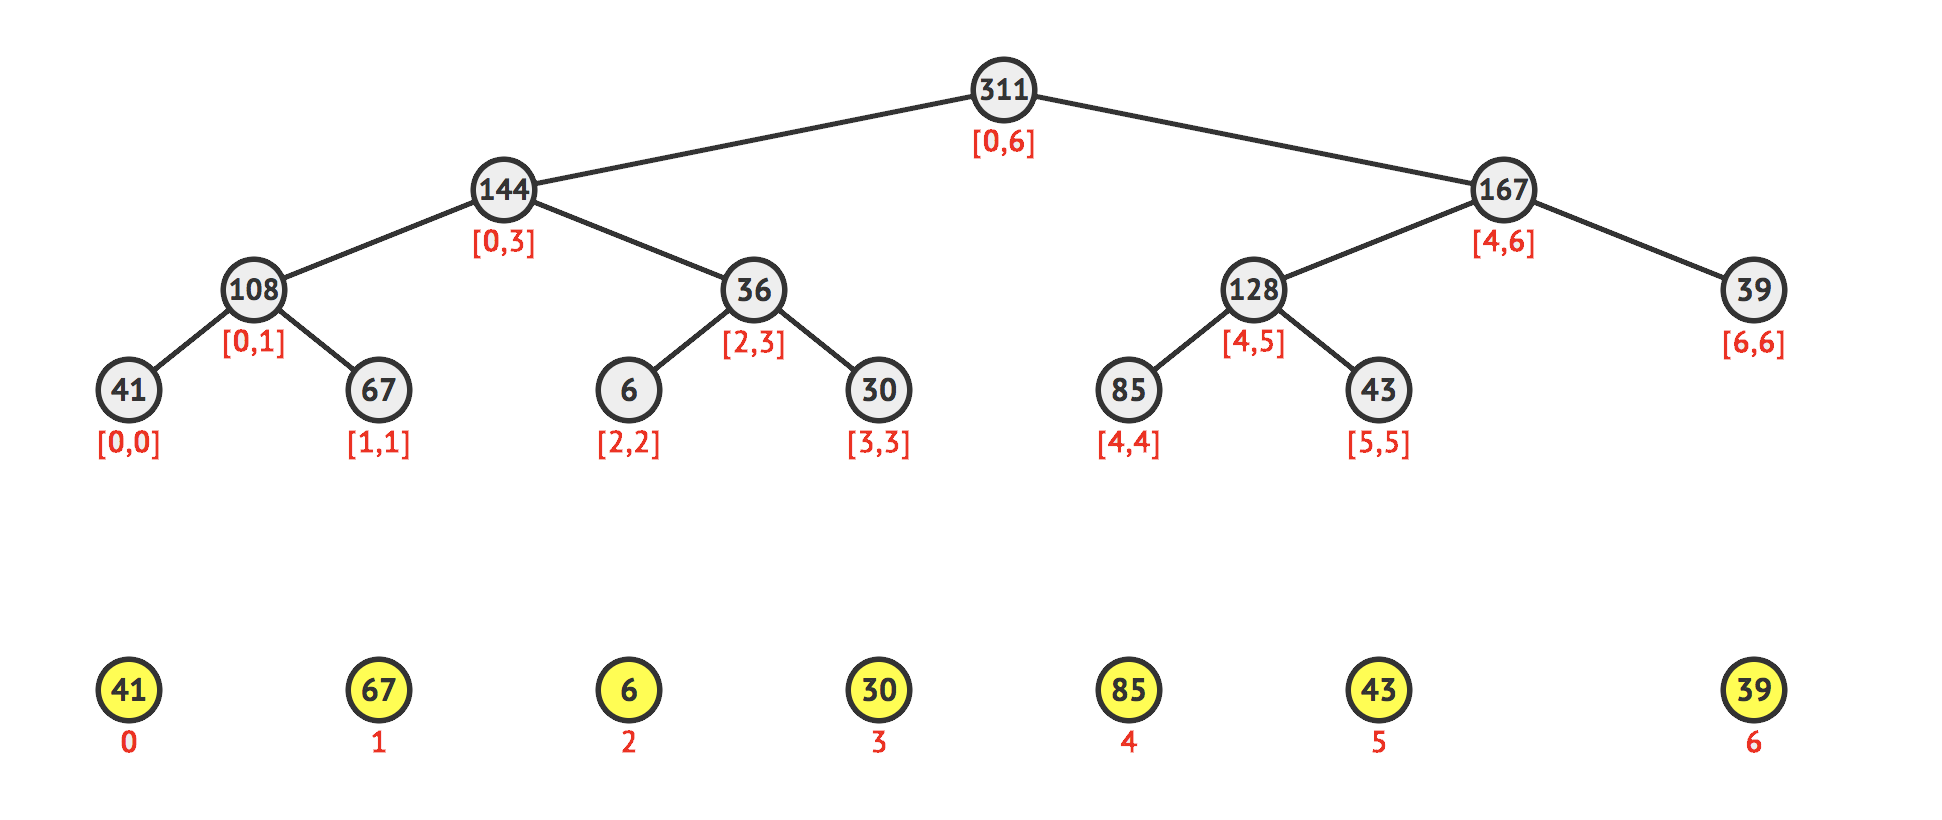
\includegraphics[width=\linewidth/1]{segtree.png}
		\label{fig:segtree}
        \caption{
        $a = [41,67,6,30,85,43,39]$ dizisinde toplam sorgusu icin olu\c{s}turulmu\c{s} segment tree yap{\i}s{\i}}
	\end{figure}
	
	\clearpage
	
    \begin{minted}[frame=lines,linenos,fontsize=\footnotesize]{c++}

void build(int ind,int l,int r) {
  // tree[ind] dizinin [l,r] araliginin cevabini saklar.

  if (l == r) { // yaprak dugum'e ulasti
    tree[ind] = a[l]; //bu dugum dizinin l. elamaninin cevabini saklar
  }
  else {
    int mid = (l + r) / 2;
    build(ind * 2,l,mid);
    build(ind * 2 + 1,mid + 1,r);
    // [l,r] araliginin cevabini
    // [l,mid] ve [mid + 1,r] araliklarinin cevaplarinin birlesmesiyle olusur.
    tree[ind] = tree[ind * 2] + tree[ind * 2 + 1];
  }
  return;
}

    \end{minted}
    
    \subsection{Aral{\i}k Sorgu ve Eleman G\"{u}ncelleme}
    
    \subsubsection{Sorgu Algoritmas{\i}}
    
    Herhangi bir $[l,r]$ aral{\i}\u{g}{\i} i\c{c}in sorgu algoritmas{\i} s{\i}ras{\i} ile \c{s}u \c{s}ekilde \c{c}al{\i}\c{s}{\i}r:
    
    \begin{itemize}
        
        \item $[l,r]$ aral{\i}\u{g}{\i}n{\i} a\u{g}ac{\i}m{\i}zda cevaplar{\i} sakl{\i} olan en geni\c{s} aral{\i}klara  par\c{c}ala.
        
        \item Bu aral{\i}klar{\i}n cevaplar{\i}n{\i} birle\c{s}tirerek istenilen cevab{\i} hesapla.
    
    \end{itemize}

    A\u{g}ac{\i}n her derinli\u{g}inde cevab{\i}m{\i}z i\c{c}in gerekli aral{\i}klardan maksimum 2
    adet bulunabilir. Bu y\"{u}zden sorgu algoritmas{\i} $O(logN)$ zaman karma\c{s}{\i}kl{\i}\u{g}{\i}nda \c{c}al{\i}\c{s}{\i}r.

    
    \clearpage
    
	\begin{figure}[h]
		\centering
		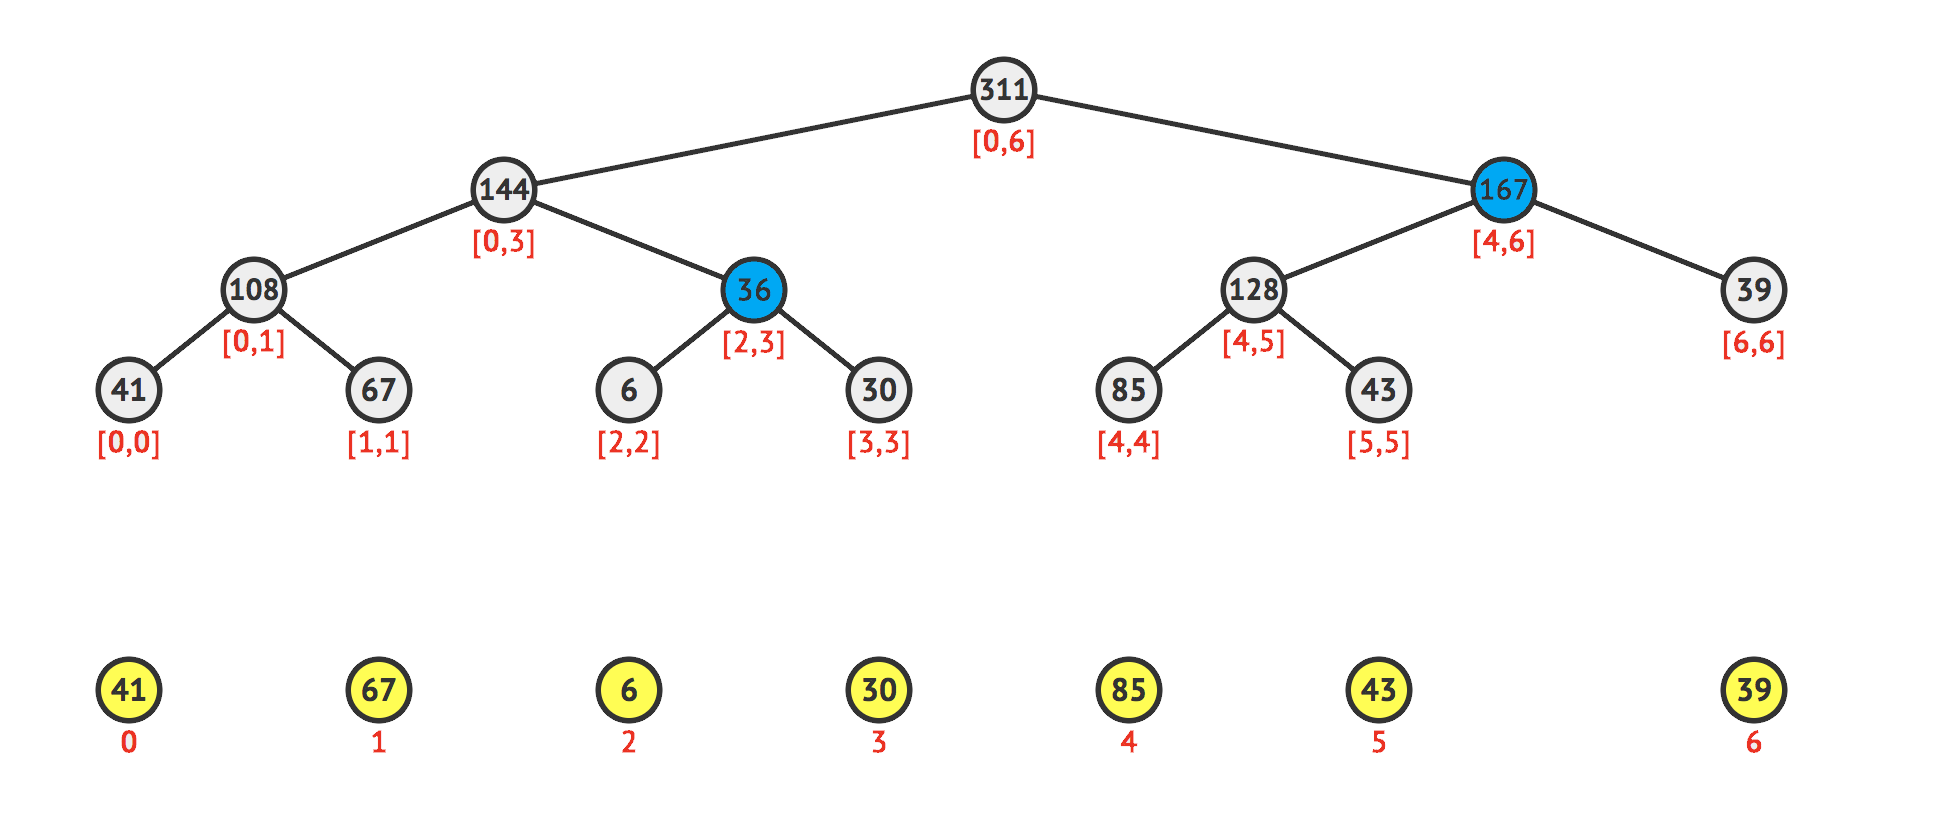
\includegraphics[width=\linewidth/1]{segtreequery.png}
		\label{fig:segtreequery}
        \caption{$a = [41,67,6,30,85,43,39]$ dizisinde $[2,6]$ aral{\i}\u{g}{\i}nda sorgu i\c{s}lemi}
	\end{figure}

    $a = [41,67,6,30,85,43,39]$ dizisinde [2,6] aral{\i}\u{g}{\i}n{\i}n cevab{\i} $[2,3]$ ile $[4,6]$ aral{\i}klar{\i}n{\i}n cevaplar{\i}n{\i}n birle\c{s}mesiyle elde edilir. Toplam sorgusu i\c{c}in cevap $36+167=203$ \c{s}eklinde hesaplan{\i}r.
    
    \begin{minted}[frame=lines,linenos,fontsize=\footnotesize]{c++}

// [lw,rw] sorguda cevabini aradigimiz aralik.
// [l,r] ise agactaki ind nolu node'da cevabini sakladigimiz aralik.

int query(int ind,int l,int r,int lw,int rw) { 
  if (l > rw or r < lw) //bulundugumuz aralik cevabini aradigimiz araligin disinda.
    return 0;
  if (l >= lw and r <= rw) //cevabini aradigimiz aralik bu araligi tamamen kapsiyor.
    return tree[ind];
  int mid = (l + r) / 2;
  //Agacta recursive birseklide araligimizi
  // araliklara bolup gelen cevaplari birlestiyoruz.  
  return query(ind * 2,l,mid,lw,rw) + query(ind * 2 + 1,mid + 1,r,lw,rw);
}
    
    \end{minted}    
    
    \subsubsection{Eleman G\"{u}ncelleme Algoritmas{\i}}
    
    Dizideki $x$ indeksli eleman{\i}n{\i}n de\u{g}erini g\"{u}ncellemek i\c{c}in kullan{\i}lan algoritma \c{s}u \c{s}eklide \c{c}al{\i}\c{s}{\i}r.
    
    \begin{itemize}
        \item A\u{g}a\c{c}ta $x$ indeksli eleman{\i} i\c{c}eren tum d\"{u}\u{g}\"umlerin de\u{g}erlerini g\"{u}ncelle.
    \end{itemize}
    
    A\u{g}a\c{c}ta x indeksli eleman{\i}n cevab{\i}n{\i} tutan yaprak d\"{u}\u{g}\"{u}mden root d\"{u}\u{g}\"{u}me kadar toplamda $logN$ d\"{u}\u{g}\"{u}m\"{u}n de\u{g}erini g\"{u}ncellememiz yeterlidir. Dolay{\i}s{\i}yla herhangi bir eleman{\i}n de\u{g}erini g\"{u}ncellemenin zaman karma\c{s}{\i}kl{\i}\u{g}{\i} $O(logN)$'dir.
    
	\begin{figure}[h]
		\centering
		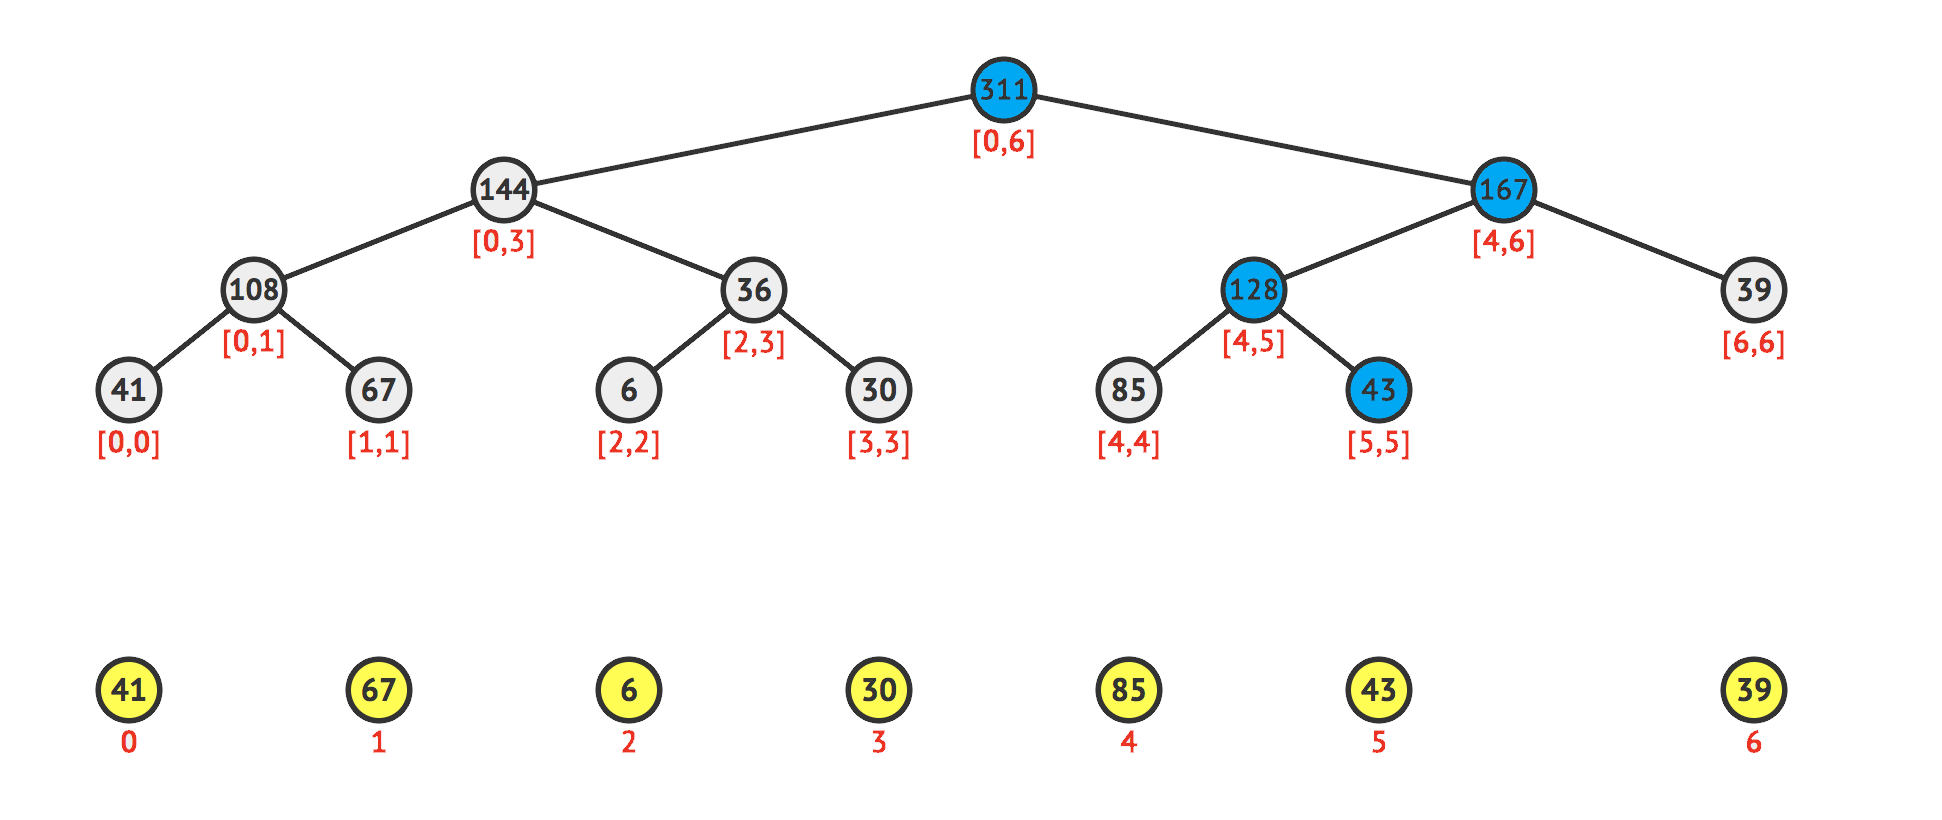
\includegraphics[width=\linewidth/1]{segtreeupdate.png}
		\label{fig:segtreeupdate}
        \caption{$a = [41,67,6,30,85,43,39]$ dizisinde 5 indeksli eleman{\i}n cevab{\i}n{\i} g\"{u}ncellerken g\"{u}ncellememiz gereken d\"{u}\u{g}\"{u}mler sekildeki gibidir.}
	\end{figure}
    
    \begin{minted}[frame=lines,linenos,fontsize=\footnotesize]{c++}

void update(int ind,int l,int r,int x,int val) {
  if (l > x || r < x) //bulundugumuz aralik x indeksli elemani icermiyor.
    return;
  if (l == x and r == x) {
    tree[ind] = val; //x indeksli elemani iceren yaprak dugumunun cevabini guncelliyoruz.
    return;
  }
  int mid = (l + r) / 2;
  // recursive bir sekilde x indeksli elemani iceren
  // tum araliklarin cevaplarini guncelliyoruz.
  update(ind * 2,l,mid,x,val);
  update(ind * 2 + 1,mid + 1,r,x,val);
  tree[ind] = tree[ind * 2] + tree[ind * 2 + 1];
}

    \end{minted}
    Segment Tree veri yap{\i}s{\i} ile ilgili problem: \href{https://codeforces.com/gym/100739/problem/A}{Link}.
    \cleardoublepage
    
    \section{\"{O}rnek Problemler}
    
    Veri yap{\i}lar{\i} \"{u}zerinde pratik yapabilmeniz i\c{c}in \"{o}nerilen problemler :
    \begin{enumerate}
        \item \href{https://codeforces.com/problemset/problem/797/C}{Link}
        \item \href{https://codeforces.com/contest/276/problem/C}{Link}
        \item \href{https://codeforces.com/contest/380/problem/C}{Link}
        \item \href{https://www.hackerearth.com/problem/algorithm/benny-and-sum-2/}{Link}
        \item \href{https://www.hackerearth.com/practice/data-structures/advanced-data-structures/fenwick-binary-indexed-trees/practice-problems/algorithm/counting-in-byteland/}{Link}
    \end{enumerate}
    
    \newpage
    
    \begin{thebibliography}{2}
    
    \bibitem{1}
    
    https://en.wikipedia.org/wiki/Data\_structure    

    \bibitem{2}
    https://cp-algorithms.com/data\_structures/sparse-table.html

    \bibitem{3}
    https://cp-algorithms.com/data\_structures/segment\_tree.html
    
    \bibitem{4}
    https://cp-algorithms.com/data\_structures/fenwick.html
  
    \bibitem{5}
    https://cp-algorithms.com/data\_structures/sqrt\_decomposition.html
    
    \bibitem{6}
    https://cses.fi/book/book.pdf
    
    \bibitem{7}
    https://visualgo.net/en/segmenttree
    
    \bibitem{8}
    https://visualgo.net/en/fenwicktree
    
    \bibitem{9}

    https://www.geeksforgeeks.org/binary-indexed-tree-or-fenwick-tree-2/
    
    \bibitem{10}
    
    http://www.cs.ukzn.ac.za/~hughm/ds/slides/20-stacks-queues-deques.pdf
    
    \bibitem{11}
    
    https://www.geeksforgeeks.org/stack-data-structure/    
    
    \bibitem{12}
    
    https://www.geeksforgeeks.org/queue-data-structure/
    
    \bibitem{13}
    
    https://www.geeksforgeeks.org/deque-set-1-introduction-applications/    
    
    \bibitem{14}
    
    https://www.geeksforgeeks.org/linked-list-set-1-introduction/
    
    \bibitem{15}
    
    https://www.geeksforgeeks.org/binary-indexed-tree-range-updates-point-queries/
    
    \bibitem{16}
    
    https://visualgo.net/en/list    
    
    \end{thebibliography} 

 \end{document}